\documentclass[11pt,a4paper]{article}
\usepackage[utf8]{inputenc}
\usepackage[french]{babel}
\usepackage[T1]{fontenc}
\usepackage{graphicx}
\usepackage{lmodern}
\usepackage{mathtools}
\usepackage{amssymb}

\begin{document}
\title{Heroes of Ponts \& Chaussées \\ Manuel d'Utilisation}
\author{Charles AUGUSTE, Nathanaël GROSS-HUMBERT, Clément RIU, Anne SPITZ}
\maketitle

Faute de temps, notre projet se compose actuellement de deux programmes distincts : une partie ``fonctionnelle'' avec des graphismes sommaires, et une partie ``Graphique'' qui comprend une gestion d'une carte beaucoup plus grande, un déplacement de la carte au clavier et sur la mini-map, mais qui ne permet pas de jouer.

\section{Partie Gestion}

Nous avons créé un projet très général. Ainsi, beaucoup de fonctionnalités pourraient être implémentées en plus. En l'état, le but du jeu est assez sommaire : tuer les héros ennemis. \\
Le jeu est pour l'instant à 2 joueurs, mais est destiné à être jouable contre une IA.

\subsection{Le principe du jeu}

Vous possédez des héros sur la carte principale (voir figure~\ref{fig2}). Ce sont les carrés de couleur avec de petits carrés blancs à  l'intérieur. Chaque tour, vous pouvez les déplacer, les faire entrer dans des villes alliées (où ils pourront acheter de l'équipement) ou les faire attaquer. Lorsque vous terminez votre tour (en cliquant sur "fin de tour"), c'est à l'ennemi de jouer. \\
L'objectif est de détruire tous les héros ennemis. \\
\\
Pour ce faire, déplacez-vous jute à côté d'un héros ennemi, puis cliquez sur lui. Vous entrerez alors dans la phase de combat et une carte aléatoire sera alors générée grâce à l'algorithme du recuit simulé. Vous pourrez alors vous battre avec les héros combattants et leur sbires. Pour gagner le combat, tuez le Héros ennemi, les sbires fuiront. Vous serez alors ramenés à la carte principale.

\subsection{Ce qui est fonctionnel}

\subsubsection{Écran d'ouverture}

Cliquez sur "Nouvelle Partie" pour commencer une nouvelle partie avec des positions de départ prédéfinies.

Cliquez sur "Charger Partie" pour charger une partie sauvegardée ; pour l'instant la sauvegarde ne garde en mémoire que la position des deux héros bleus.

\begin{figure}[h]
\begin{center}
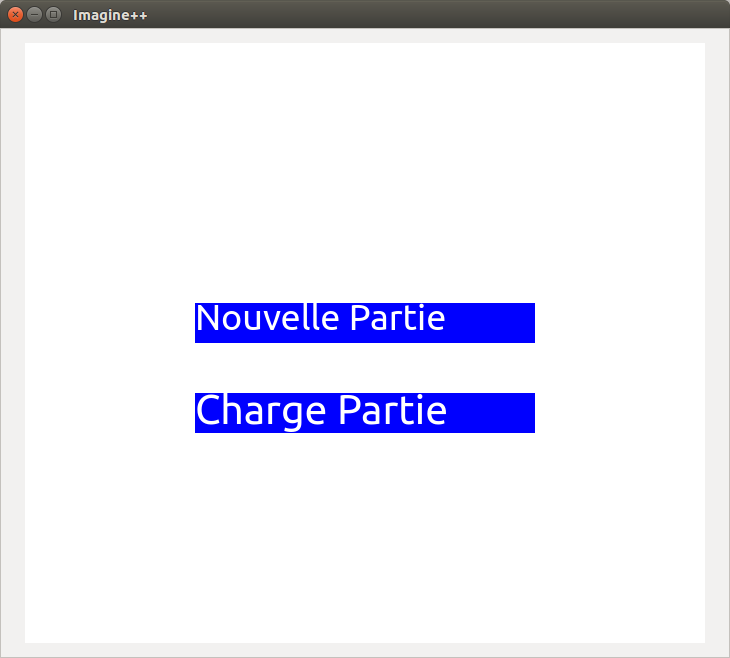
\includegraphics[scale=0.5]{./ecran_de_demarrage.png}
\caption{Écran de démarrage}
\end{center}
\end{figure}

\clearpage

\subsubsection{Écran de jeu}


\begin{figure}[h]
\begin{center}
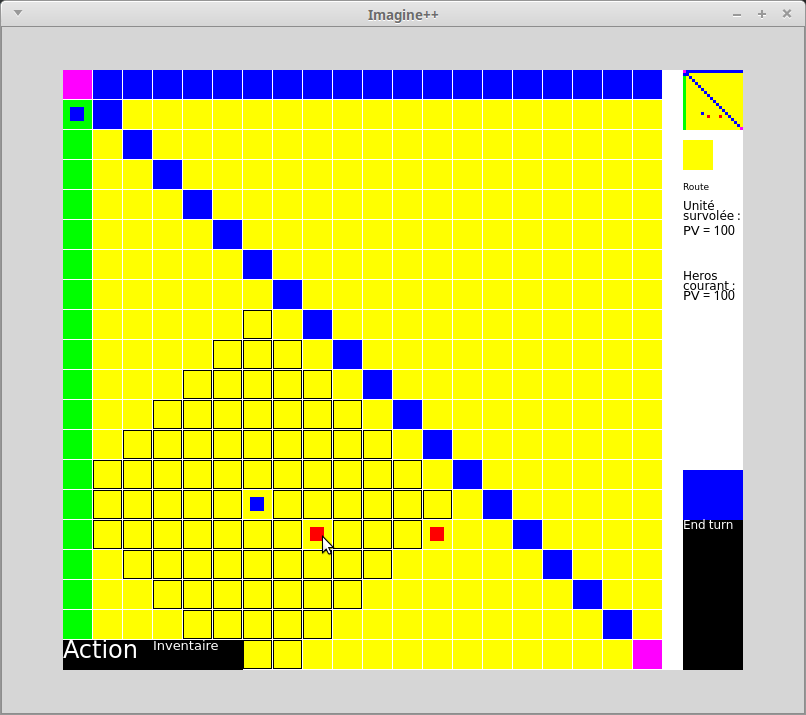
\includegraphics[scale=0.5]{./ecran_de_gestion.png}
\caption{Écran de jeu principal\label{fig2}}

\end{center}
\end{figure}

La plus grande partie de l'écran se compose de la carte principale. La droite de l'écran correspond à la barre d'outil, qui permet notamment de : finir son tour, sauvegarder \& quitter, afficher le nombre PV des unités survolées et de celle sélectionnée, afficher le numéro du tour et le joueur dont c'est le tour, et la mini-carte (qui affiche une vue d'ensemble à taille réduite de la carte totale. Pour l'instant, toute la carte est visible mais elle est destinée à être plus large, comme dans la partie graphique). \\

Les différentes couleurs de cases correspondent à des types de cases différentes : \\
\begin{itemize}
\item Une case bleue correspond à de l'eau, infranchissable ;
\item Une case jaune correspond à une route, à moindre coût de déplacement ;
\item Une case verte correspond à des champs, qui sont deux fois plus longs à traverser que les routes ;\
\item Une case violette correspond à une ville (ennemie ou alliée, indifférencié pour l'instant) ;
\item On peut rajouter très facilement d'autres types de cases, mais nous ne désirions pas complexifier le jeu plus que nécessaire.
\end{itemize}

La description des cases s'affiche en-dessous de la minicarte.

Les boutons "Save \& Quit" et "End turn" :\\
Cliquez sur "Save \& Quit" pour sauvegarder le jeu et pouvoir le charger plus tard (pour l'instant, seules les positions des deux héros bleus sont sauvegardées).
Cliquez sur "End turn" pour mettre fin au tour.\\

Les unités sur la carte sont représentées par des carrés bleus ou rouge selon le joueur auquel elles appartiennent. \\
Cliquez sur une unité pour la sélectionner. Les cases que l'unité peut atteindre apparaissent cerclées de noir. On peut se déplacer tant qu'il reste des points de déplacement.

Notez que vous ne pouvez déplacer que les unités bleues ou rouges. Les unités restantes sont celles de l'autre joueur et ne pourront pas se déplacer tant que vous n'aurez pas cliqué sur ``fin de tour''. \\
\\

Lorsqu'une unité se situe sur une case adjacente à une unité appartenant au joueur adverse, elle peut attaquer cette unité. Pour cela, sélectionnez l'unité et cliquez avec le bouton gauche de la souris sur l'unité que vous souhaitez attaquer. Cette action déclenche la partie combat.

Lorsqu'une unité se situe sur une case adjacente à une ville (cases roses) appartenant au même joueur, elle peut rentrer dans la ville pour afficher l'écran d'achat. Pour cela, sélectionnez l'unité puis cliquez sur la ville avec le bouton gauche de la souris. Un écran s'ouvrira alors pour vous demander confirmation.

Lorsqu'une unité est sélectionnée, les boutons "action" et "inventaire" apparaissent en bas à gauche de l'écran.
Le bouton "action" n'est pas encore fonctionnel.
Le bouton "inventaire" ouvre l'inventaire.

\clearpage

\subsubsection{Écran d'inventaire}

\begin{figure}[h]
\begin{center}
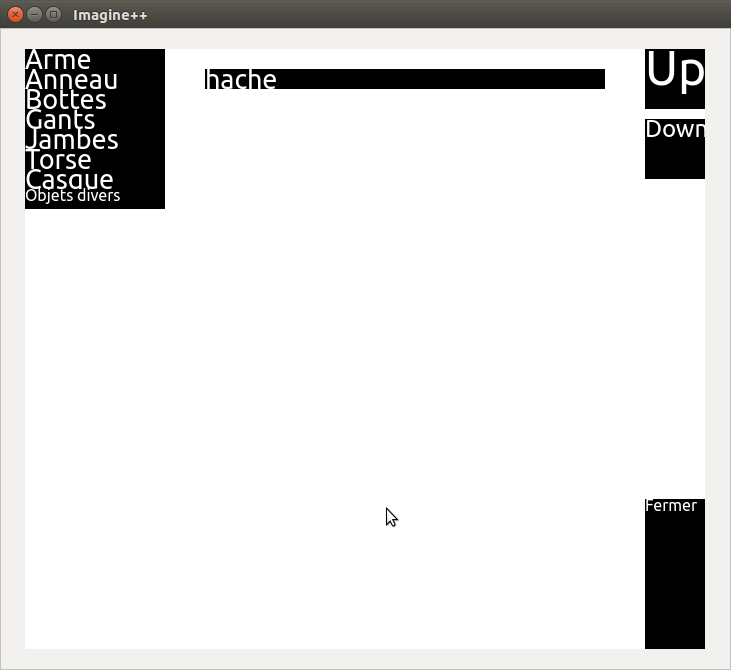
\includegraphics[scale=0.5]{./ecran_inventaire.png}
\caption{Écran d'inventaire}
\end{center}
\end{figure}

Cet écran affiche les différentes catégories d'objets équipables par une unité, ainsi qu'une rubrique "objet divers".

Cliquez sur une catégorie d'objet équipable pour afficher l'objet correspondant actuellement équipé par l'unité.
Les différents types d'objet équipables sont:
\begin{itemize}
\item Arme
\item Anneau
\item Bottes
\item Gants
\item Jambes
\item Torse
\item Casque
\end{itemize}

Cliquez sur "objet divers" pour afficher l'ensemble des objets non équipés transporté par le héros.

Cliquez sur "Up et "Down" pour faire défiler la liste d'objet.

Cliquez sur "Fermer" pour fermer l'inventaire et revenir à l'écran de jeu.

Un clic droit sur un objet quelconque permettra d'afficher ses caractéristiques. Il faudra alors cliquer de nouveau pour ré afficher le menu de l'inventaire. 

\begin{figure}[h]
\begin{center}
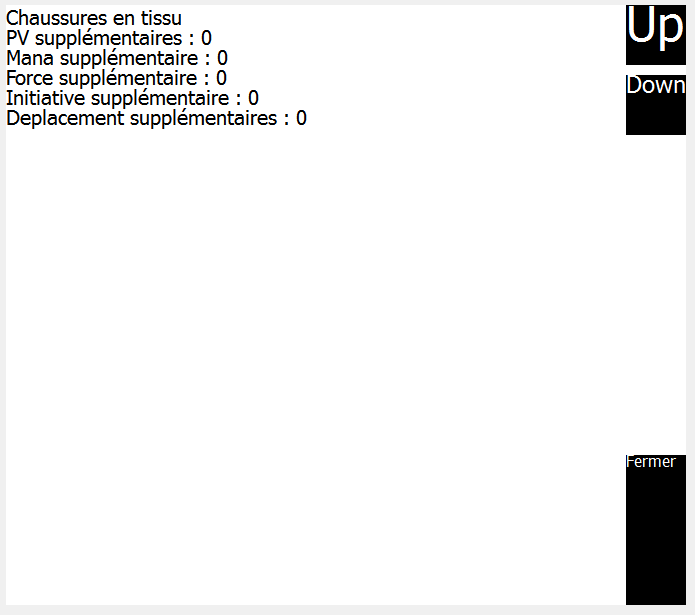
\includegraphics[scale=0.5]{./ecran_carac_objet.png}
\caption{Écran de caractéristiques des objets}
\end{center}
\end{figure}

\subsubsection{Écran d'achat}

\begin{figure}[h]
\begin{center}
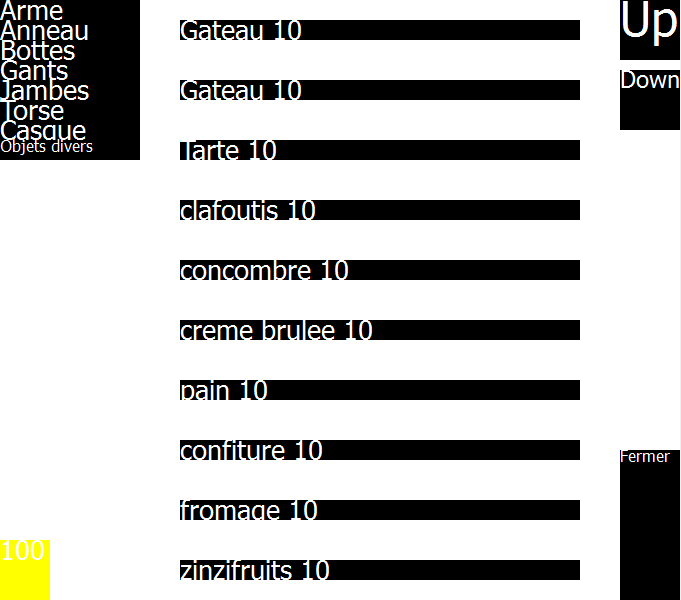
\includegraphics[scale=0.6]{./ecranAchat.png}
\caption{Écran d'achat}
\end{center}
\end{figure}

Cet écran s'affiche lorsqu'une unité rentre dans une ville.

Cet écran est similaire à l'écran d'inventaire, sauf que les objets affiché ne sont pas ceux transporté par le héros mais ceux disponibles au marché de la ville.

Cliquez sur un objet pour que celui-ci s'ajoute à l'inventaire du héros.

Encore une fois, un clic droit sur un objet de la boutique permettra d'afficher les caractéristiques de la boutique.

\subsection{Ce que nous allons implémenter}

Les graphismes seront affiché avec les fonctionnalités de la partie Graphisme. \\
Il sera possible de gérer la croissance des villes, de construire des bâtiments permettant de recruter différents types de sbires. Les soldats et objets disponibles dans les villes pourront changer en fonction du développement de celle-ci.

Il sera possible de stocker plusieurs sauvegardes de manière simultanée, et les sauvegardes permettront de tout sauvegarder (pour l'instant, la sauvegarde ne gère que les deux héros bleus).


\section{Partie Combat}

\subsection{Ce qui est fonctionnel}

\begin{figure}[h]
\begin{center}
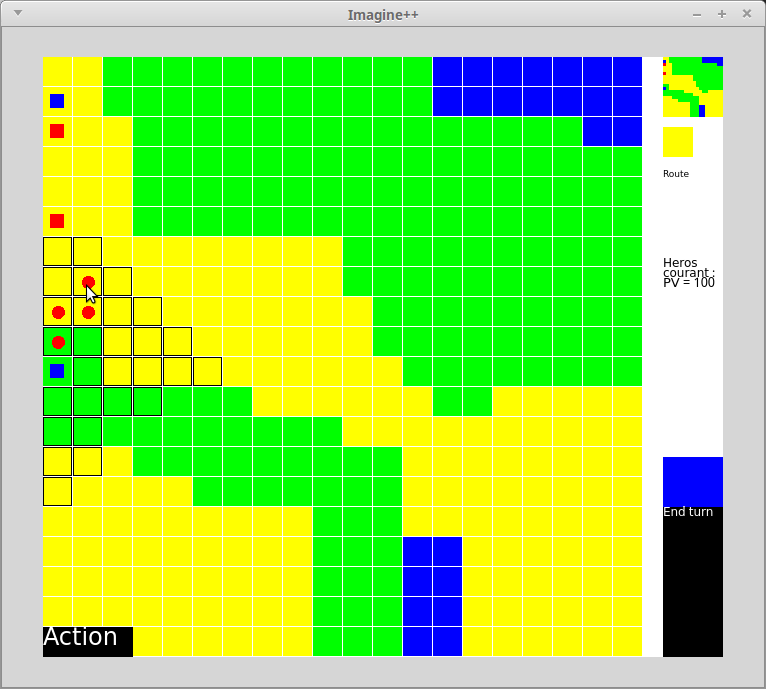
\includegraphics[scale=0.5]{./ecran_de_combat.png}
\caption{Écran de combat}
\end{center}
\end{figure}


Cette partie est déclenchée par la partie gestion lorsqu'une unité en attaque une autre.

La plus grande partie de l'écran se compose de la carte principale. Celle-ci est généré aléatoirement à chaque combat. Les unités apparaissent pour l'instant à des endroits prédéfinis (mais ne tomberont jamais dans l'eau), à l'avenir il sera possible de les placer avant le début du combat. \\
L'interface est identique à celle de gestion. \\

Contrairement à la phase gestion, vous ne choisissez pas quelle unité vous contrôlez ; l'ordre dans lequel elles jouent est déterminé par une file de priorité en fonction de leur ``initiative'' (une statistique liée à l'unité).\\

Après s'être déplacée, si elle ne s'est pas déplacée du nombre de case maximum possible, elle peut encore se déplacer. Lors des déplacements, le chemin le plus court que va prendre l'unité s'affiche avec des ronds rouges.

Lorsqu'une unité est active, le bouton "action" apparaît en bas à gauche de l'écran.

Le bouton "action" permet d'attaquer l'ennemi, cliquer dessus fait apparaître des cadres noirs dans les cases où l'unité peut attaquer. Lorsqu'une unité est attaqué, elle perd des points de vie. Lorsque ses points de vie tombe à zéro, elle meurt. Si cette unité était un héros, le joueur contrôlant cette unité perd le combat et le combat est fini.

Pour attaquer une unité, on peut aussi cliquer dessus lors d'une phase de déplacement. On va alors se coller à elle et effectuer une attaque de base. On se placera différemment en fonction de l'endroit où l'on clique sur l'unité. Dans tous les cas, le chemin que prendra l'unité est affiché en rouge.

On ne peut plus accéder à l'inventaire dans la phase combat.

\subsection{Ce que nous allons implémenter}

-Les fonctionnalités graphiques utilisée seront celles de la partie graphique. \\
-Il sera possible de choisir les positions de départ des unités \\
-Il existera plusieurs types de sbires (comme des archers, des cavaliers...) ayant des caractéristiques et des intérêts stratégiques différents.

\clearpage

\section{Partie Graphique}

Cette partie contient principalement les fonctions graphiques qui seront utilisée dans les autres parties. \\
Pour la lancer, compilez le projet ``Affichage'' présent dans le dossier du même nom.

\subsection{Écran de démarrage}

\begin{figure}[h]
\begin{center}
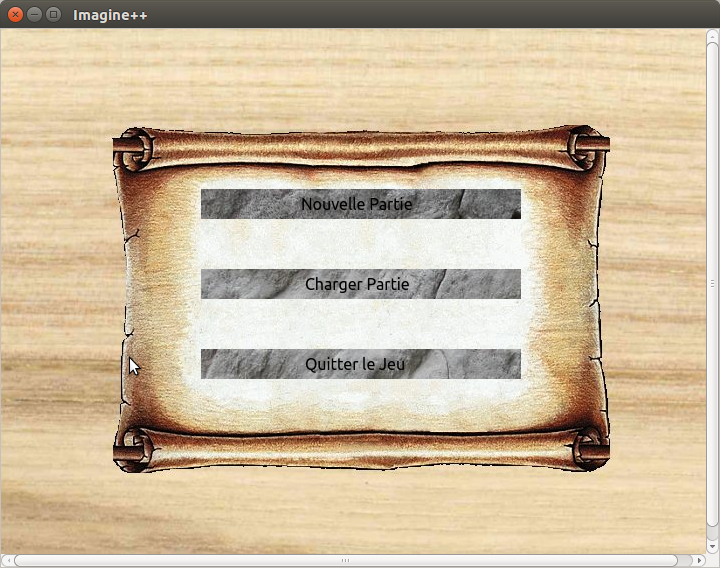
\includegraphics[scale=0.5]{./graphique_demarrage.png}
\caption{Écran de démarrage}
\end{center}
\end{figure}

\clearpage


\subsection{Écran principal}

\begin{figure}[h]
\begin{center}
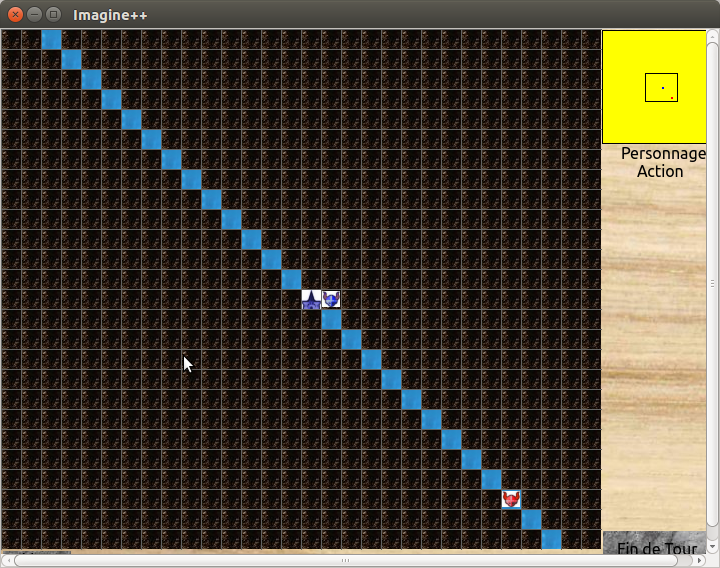
\includegraphics[scale=0.5]{./graphique_principal.png}
\caption{Écran principal}
\end{center}
\end{figure}

La principale nouveauté de cette partie est que la carte principale est bien plus grande que la partie affichée à l'écran. La partie affichée est indiquée sur la minicarte par un cadre noir. On peut modifier la partie de la carte principale affichée à l'écran en appuyant sur les touches fléchées, ou en cliquant sur la minicarte.
~~

En bas à gauche se situe le bouton "Menu" qui ouvre le menu de jeu. Les boutons ne sont pas encore fonctionnels.

\end{document}